\section{Existence and Uniqueness of Solutions of Nonlinear Equations}

\noindent
Although  there are  methods for
 solving some nonlinear equations, it's
impossible to find  useful formulas for the solutions of most.
Whether we're looking for  exact solutions or numerical
approximations, it's useful to know  conditions that imply the
existence and uniqueness of solutions of initial value problems for
nonlinear equations. In this section we state  such a condition and
illustrate it with examples.

\vspace*{-15pt}
\begin{figure}[H]
  \centering
\scalebox{.9}{
  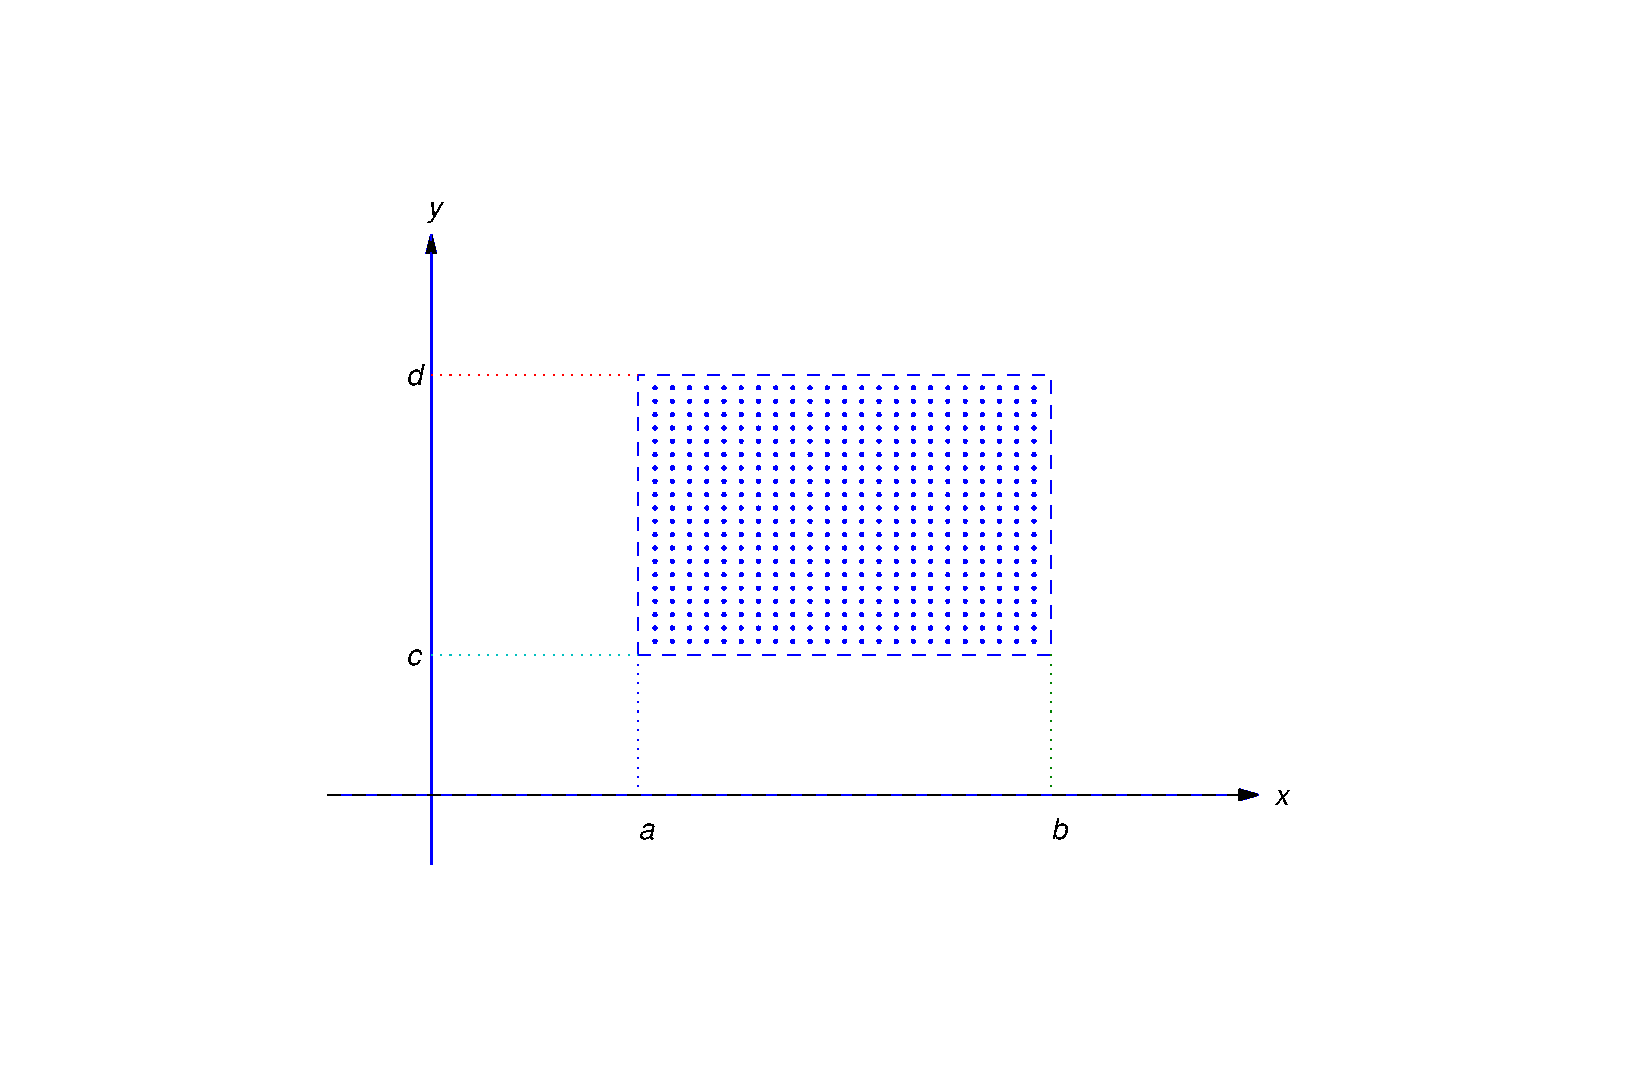
\includegraphics[bb=-78 148 689 643,width=5.67in,height=3.66in,keepaspectratio]{fig020301}}
\color{blue}
\vspace*{-35pt}
  \caption{An open rectangle}
  \label{figure:2.3.1}
\end{figure}

Some terminology:
 an {\color{blue}\it open rectangle $R$\/}
 is a set of points $(x,y)$ such that
$$
a<x<b\mbox{\quad  and \quad}c<y<d
$$
 (Figure~\ref{figure:2.3.1}).  We'll denote this set by
$R:  \{ a < x < b, c < y < d \}$.
 ``Open'' means that the
boundary rectangle (indicated by the dashed lines in
Figure~\ref{figure:2.3.1}) isn't  included in  $R$ .

The next theorem gives sufficient conditions for existence and
uniqueness of solutions of initial value problems for first order
nonlinear differential equations. We omit the proof, which is beyond
the scope of this book.

\begin{theorem}\color{blue} \label{thmtype:2.3.1} \mbox{}\newline
\vspace*{-5pt}
\begin{alist}
\item %(a)
 If  $f$ is continuous
on an open rectangle
$$
R:  \{ a < x < b, c < y < d \}
$$
 that contains $(x_0,y_0)$
then  the initial value problem
\begin{equation} \label{eq:2.3.1}
y'=f(x,y), \quad y(x_0)=y_0
\end{equation}
 has at least one solution  on some open subinterval
of  $(a,b)$ that contains $x_0$.

\item % (b)
 If  both $f$ and  $f_y$ are
 continuous on $R$ then \eqref{eq:2.3.1} has a unique
solution on some open subinterval  of $(a,b)$ that contains $x_0$.
\end{alist}
\end{theorem}

It's important to understand exactly what Theorem~\ref{thmtype:2.3.1}
says.

\begin{itemize}
\item \part{a} is an {\color{blue}\it existence theorem\/}. It guarantees that a
solution exists on some open interval that contains $x_0$, but provides
no information on how to find the solution, or to determine the open
interval on which it exists. Moreover, \part{a} provides no
information on the number of solutions that \eqref{eq:2.3.1} may have. It
leaves open the possibility that \eqref{eq:2.3.1} may have two or more
solutions that differ for values of $x$ arbitrarily close to $x_0$. We
will see in Example~\ref{example:2.3.6} that this can happen.

\item \part{b} is a {\color{blue}\it uniqueness theorem\/}. It guarantees that
\eqref{eq:2.3.1} has a unique solution on some open interval (a,b) that
contains $x_0$. However, if $(a,b)\ne(-\infty,\infty)$,
\eqref{eq:2.3.1} may have more than one solution on a larger interval
that contains $(a,b)$. For example, it may happen that $b<\infty$ and all
solutions have the same values on $(a,b)$, but two solutions $y_1$ and
$y_2$ are defined on some interval $(a,b_1)$ with $b_1>b$, and have
different values for $b<x<b_1$;   thus, the graphs of the $y_1$ and
$y_2$ ``branch off'' in different directions at $x=b$. (See
Example~\ref{example:2.3.7} and Figure~\ref{figure:2.3.3}). In this case,
continuity implies that $y_1(b)=y_2(b)$ (call their common value
$\overline y$), and  $y_1$ and $y_2$ are both solutions of the initial
value problem
\begin{equation} \label{eq:2.3.2}
y'=f(x,y),\quad y(b)=\overline y
\end{equation}
that differ on every open interval that contains $b$. Therefore
$f$ or $f_y$ must have a discontinuity at some point in each open
rectangle that contains $(b,\overline y)$, since if this were not so,
\eqref{eq:2.3.2} would have a unique solution on some open interval
that contains $b$. We leave it to you to give a similar analysis of the
case where $a>-\infty$.
 \end{itemize}

\begin{example}\label{example:2.3.1}
\rm   Consider  the initial value problem
\begin{equation} \label{eq:2.3.3}
y'={x^2-y^2 \over 1+x^2+y^2}, \quad y(x_0)=y_0.
\end{equation}
Since
$$
f(x,y)  = {x^2-y^2 \over 1+x^2+y^2}\mbox{\quad and \quad}
f_y(x,y)  =  -{2y(1+2x^2)\over (1+x^2+y^2)^2}
$$
are continuous for all $(x,y)$, Theorem~\ref{thmtype:2.3.1} implies that
if $(x_0,y_0)$ is arbitrary, then
\eqref{eq:2.3.3} has a unique solution on some open interval that contains
$x_0$.
\end{example}

\begin{example}\label{example:2.3.2}
\rm  Consider  the initial value problem
\begin{equation} \label{eq:2.3.4}
y'={x^2-y^2 \over x^2+y^2}, \quad y(x_0)=y_0.
\end{equation}
Here
$$
f(x,y)  =  {x^2-y^2 \over x^2+y^2}\mbox{\quad and \quad}
f_y(x,y)  =  \dst -{4x^2y \over (x^2+y^2)^2}
$$
are continuous everywhere except at $(0,0)$. If $(x_0,y_0)
\ne(0,0)$, there's an open rectangle $R$ that contains
$(x_0,y_0)$ that does not contain $(0,0)$. Since $f$ and $f_y$ are
continuous on $R$, Theorem~\ref{thmtype:2.3.1} implies that if
$(x_0,y_0)\ne(0,0)$ then
\eqref{eq:2.3.4}
has a unique solution on some open interval that contains $x_0$.
\end{example}

\begin{example}\label{example:2.3.3}
\rm  Consider the initial value problem
\begin{equation} \label{eq:2.3.5}
y'={x+y\over x-y},\quad y(x_0)=y_0.
\end{equation}
Here
$$
f(x,y)  =  {x+y\over x-y}\mbox{\quad and \quad}
f_y(x,y)  =  {2x\over (x-y)^2}
$$
are continuous everywhere except on the line $y=x$. If $y_0\ne x_0$,
there's an open rectangle $R$ that contains $(x_0,y_0)$ that
does not intersect the line $y=x$. Since $f$ and $f_y$ are continuous
on $R$, Theorem~\ref{thmtype:2.3.1} implies that if $y_0\ne x_0$,
\eqref{eq:2.3.5} has a unique solution on some open interval that contains
$x_0$.
\end{example}

\begin{example}\label{example:2.3.4}
\rm In Example~\ref{example:2.2.4} we saw that the
solutions of
\begin{equation} \label{eq:2.3.6}
y'=2xy^2
\end{equation}
are
 $$
y\equiv0\mbox{\quad and \quad} y=-{1 \over x^2+c},
$$
where $c$ is an arbitrary constant. In particular, this implies that
no solution of \eqref{eq:2.3.6} other than $y\equiv0$ can equal zero for
any value of $x$. Show that Theorem~\ref{thmtype:2.3.1}\part{b} implies
this.
\end{example}

\solution
We'll obtain a contradiction
by assuming that \eqref{eq:2.3.6} has a solution $y_1$ that equals
zero for some value of $x$, but isn't  identically zero. If $y_1$
has this property,  there's a point $x_0$ such that $y_1(x_0)=0$,
but $y_1(x)\ne0$ for some value of $x$ in every open interval that contains
$x_0$. This means that the initial value problem
\begin{equation} \label{eq:2.3.7}
y'=2xy^2,\quad y(x_0)=0
\end{equation}
has two solutions $y\equiv0$ and $y=y_1$ that differ for some value of
$x$ on every open interval that contains $x_0$. This contradicts
Theorem~\ref{thmtype:2.3.1}(b), since in \eqref{eq:2.3.6} the functions
$$
f(x,y)=2xy^2 \mbox{\quad and \quad} f_y(x,y)= 4xy.
$$
are both continuous
for all $(x,y)$, which implies that \eqref{eq:2.3.7} has a unique
solution on some open interval that contains $x_0$.

\begin{example}\label{example:2.3.5}
\rm  Consider the initial value problem
\begin{equation} \label{eq:2.3.8}
y' = {10\over 3}xy^{2/5}, \quad y(x_0) = y_0.
\end{equation}
\begin{alist}
\item %(a)
For what points $(x_0,y_0)$ does Theorem~\ref{thmtype:2.3.1}\part{a}
imply that
\eqref{eq:2.3.8} has a solution?

\item %(b)
For what points $(x_0,y_0)$ does Theorem~\ref{thmtype:2.3.1}\part{b}
imply that
\eqref{eq:2.3.8} has a  unique solution on some open interval that contains
$x_0$?
\end{alist}
\end{example}

\solutionpart{a} Since
$$
f(x,y) = {10\over 3}xy^{2/5}
$$
is continuous for all $(x,y)$,  Theorem~\ref{thmtype:2.3.1}
implies that \eqref{eq:2.3.8} has a solution for every $(x_0,y_0)$.

\solutionpart{b} Here
$$
f_y(x,y) = {4 \over 3}xy^{-3/5}
$$
is continuous for all $(x,y)$ with $y\ne 0$. Therefore, if $y_0\ne0$
there's an open rectangle on which both $f$ and $f_y$ are
continuous, and Theorem~\ref{thmtype:2.3.1} implies that \eqref{eq:2.3.8} has
a unique solution on some open interval that contains $x_0$.

If $y=0$ then $f_y(x,y)$ is undefined, and therefore discontinuous;
hence, Theorem~\ref{thmtype:2.3.1} does not apply to \eqref{eq:2.3.8} if
$y_0=0$.

\begin{example}\label{example:2.3.6}
\rm  Example~\ref{example:2.3.5} leaves open the possibility  that the
initial value problem
\begin{equation} \label{eq:2.3.9}
y'={10 \over 3}xy^{2/5}, \quad y(0)=0
\end{equation}
has more than one solution on every open interval that contains $x_0=0$.  Show
that this is true.
\end{example}

\solution
By inspection, $y\equiv0$ is a solution of the
differential equation
\begin{equation} \label{eq:2.3.10}
y'={10 \over 3} xy ^{2/5}.
\end{equation}
 Since $y\equiv0$ satisfies the initial condition $y(0)=0$,
it's a solution of \eqref{eq:2.3.9}.

Now suppose  $y$ is a solution of \eqref{eq:2.3.10} that isn't
identically zero.
 Separating variables in \eqref{eq:2.3.10} yields
$$
 y^{-2/5}y'={10 \over 3}x
$$
on any open interval where $y$ has no zeros.
 Integrating this and rewriting the arbitrary constant as $5c/3$ yields
$$
{5\over 3}y^{3/5} = {5\over 3}(x^2+c).
$$
Therefore
\begin{equation} \label{eq:2.3.11}
y = (x^2+c)^{5/3}.
\end{equation}

Since we divided by $y$ to separate variables in \eqref{eq:2.3.10}, our
derivation of \eqref{eq:2.3.11} is legitimate only on open intervals where $y$
has no zeros. However, \eqref{eq:2.3.11} actually defines $y$ for all $x$,
and differentiating \eqref{eq:2.3.11} shows that
$$
y'={10 \over 3}x(x^2+c)^{2/3}={10 \over 3}xy^{2/5},\,-\infty<x<\infty.
$$
Therefore \eqref{eq:2.3.11} satisfies \eqref{eq:2.3.10} on
$(-\infty,\infty)$
even if $c\le 0$, so that $y(\sqrt{|c|})=y(-\sqrt{|c|})=0$. In
particular, taking $c=0$ in \eqref{eq:2.3.11} yields
$$
y=x^{10/3}
$$
as a second solution of \eqref{eq:2.3.9}.
 Both solutions are defined on
$(-\infty,\infty)$, and they differ on every
open interval that contains $x_0=0$ (see Figure~\ref{figure:2.3.2}.)
In fact, there are {\color{blue}\it four\/} distinct solutions of
\eqref{eq:2.3.9}  defined on $(-\infty,\infty)$ that differ
from each other on every open interval that contains $x_0=0$.
  Can you identify the other two?

\begin{figure}[tbp]
  \centering
  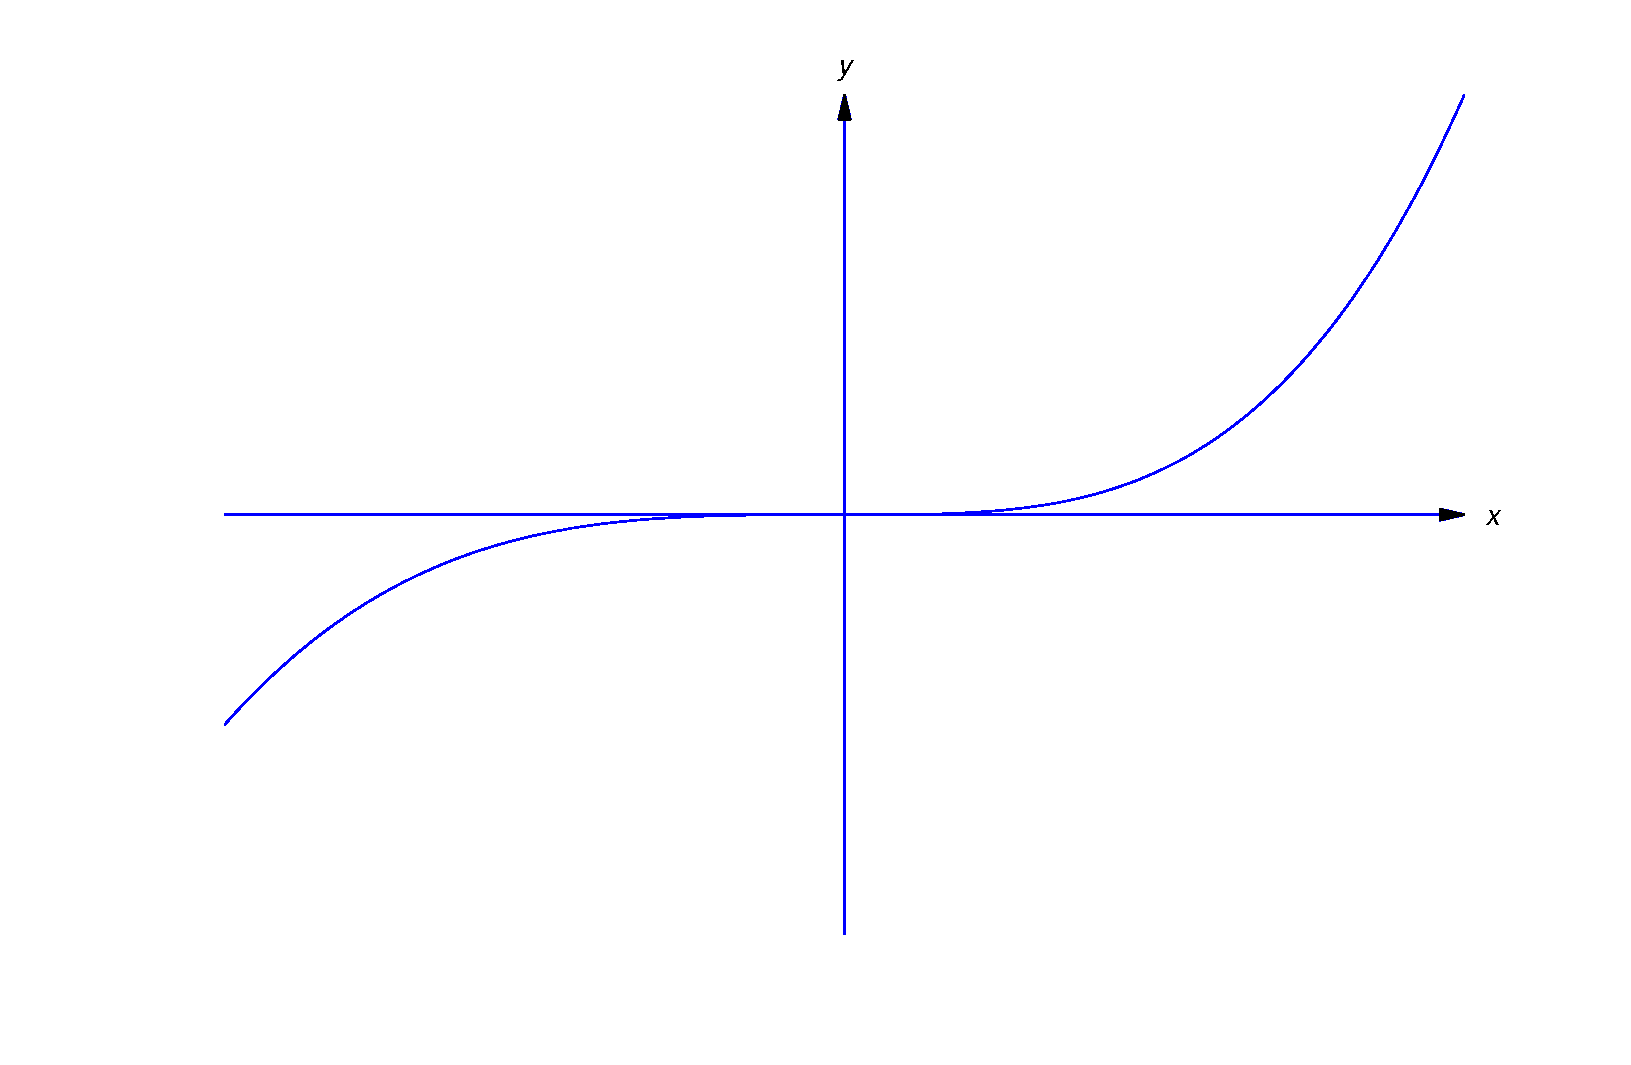
\includegraphics[bb=-78 148 689 643,width=5.67in,height=3.66in,keepaspectratio]{fig020302}
\color{blue}
\caption{Two solutions ($y=0$ and $y=x^{1/2}$) of \eqref{eq:2.3.9}  that
differ on every interval  containing $x_{0}=0$}
  \label{figure:2.3.2}
\end{figure}

\begin{example} \label{example:2.3.7}
\rm  From Example~\ref{example:2.3.5}, the initial value
problem
\begin{equation} \label{eq:2.3.12}
y'={10 \over 3}xy^{2/5}, \quad y(0)=-1
\end{equation}
 has a  unique solution on some open interval that contains $x_0=0$.
Find a solution and determine the largest open interval $(a,b)$ on
which it's unique.
\end{example}

\solution
Let $y$ be any solution of \eqref{eq:2.3.12}. Because of the initial
condition $y(0)=-1$ and the continuity of $y$, there's an open interval
$I$ that contains $x_0=0$ on which $y$ has no zeros, and is consequently
of the form \eqref{eq:2.3.11}. Setting $x=0$ and $y=-1$ in \eqref{eq:2.3.11}
yields $c=-1$, so
\begin{equation} \label{eq:2.3.13}
y=(x^2-1)^{5/3}
\end{equation}
for $x$  in $I$.
Therefore every solution of \eqref{eq:2.3.12} differs from zero
and is given by \eqref{eq:2.3.13} on $(-1,1)$; that is,
\eqref{eq:2.3.13} is the unique solution of \eqref{eq:2.3.12} on
$(-1,1)$.
 This is the largest open interval on which
\eqref{eq:2.3.12} has a unique solution. To see this, note that
\eqref{eq:2.3.13} is a solution of \eqref{eq:2.3.12} on $(-\infty,\infty)$.
From Exercise~2.2.~\hspace*{-3pt}\ref{exer:2.2.15}, there are infinitely many
other solutions
of \eqref{eq:2.3.12} that differ from \eqref{eq:2.3.13} on every open interval
larger than
$(-1,1)$. One such solution is
$$
y = \left\{ \begin{array}{cl}
(x^2-1)^{5/3}, & -1 \le x \le 1, \\[6pt]
0,             & |x|>1. \end{array} \right.
$$
(Figure \ref{figure:2.3.3}).

\begin{figure}[htbp]
\color{blue}
  \begin{minipage}[b]{0.5\linewidth}
    \centering
   \scalebox{.65}{
  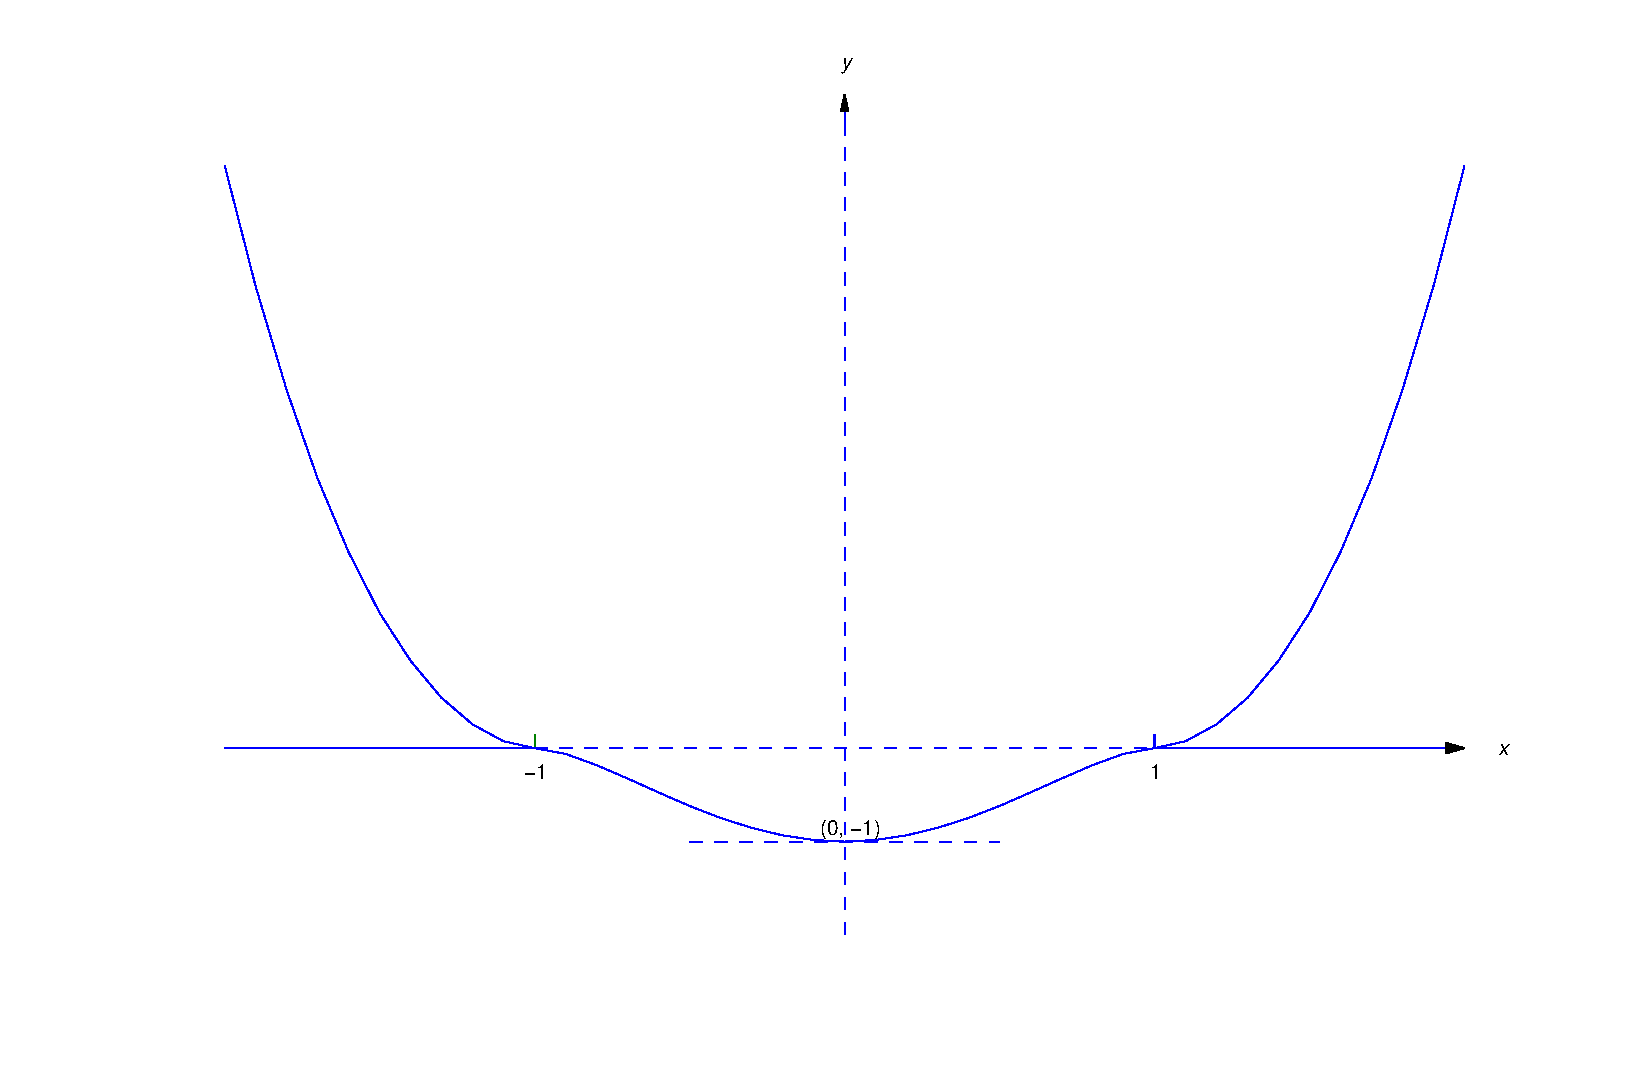
\includegraphics[bb=-78 148 689 643,width=5.67in,height=3.66in,keepaspectratio]{fig020303}}
\caption{ Two solutions of
\eqref{eq:2.3.12} on
$(-\infty,\infty)$ that coincide on $(-1,1)$, but on no larger open
interval}
  \label{figure:2.3.3}
  \end{minipage}
  \hspace{0.6cm}
  \begin{minipage}[b]{0.5\linewidth}
    \centering
   \scalebox{.65}{
  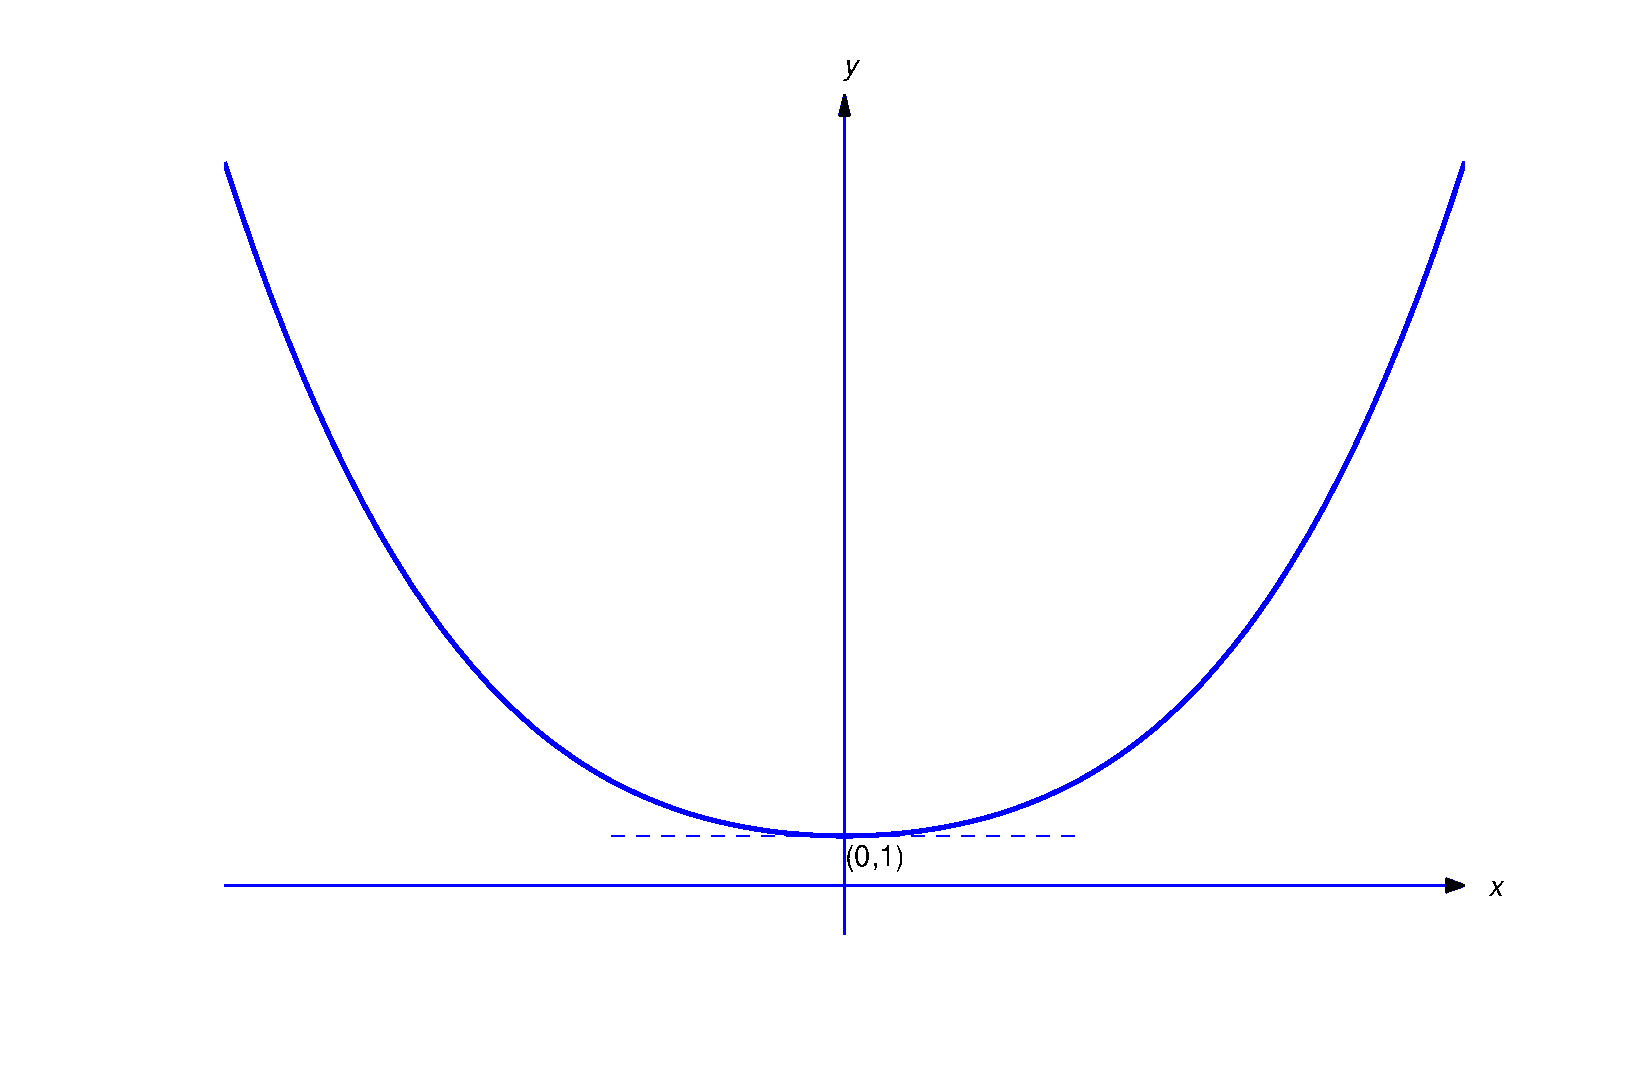
\includegraphics[bb=-78 148 689 643,width=5.67in,height=3.66in,keepaspectratio]{fig020304} }
  \caption{The unique solution of \eqref{eq:2.3.14}}
  \label{figure:2.3.4}
  \end{minipage}
\end{figure}

\begin{example}\label{example:2.3.8}
\rm  From Example~\ref{example:2.3.5}, the initial value
problem
\begin{equation} \label{eq:2.3.14}
y'={10 \over 3}xy^{2/5}, \quad y(0)=1
\end{equation}
 has a unique solution on some open interval that contains $x_0=0$.
Find the solution and determine the largest open interval on which it's
unique.
\end{example}

\solution
Let $y$ be any solution of \eqref{eq:2.3.14}. Because of the initial
condition $y(0)=1$ and the continuity of $y$, there's an open interval
$I$ that contains $x_0=0$ on which $y$ has no zeros, and is consequently
of the form \eqref{eq:2.3.11}. Setting $x=0$ and $y=1$ in \eqref{eq:2.3.11}
yields $c=1$, so
\begin{equation} \label{eq:2.3.15}
y=(x^2+1)^{5/3}
\end{equation}
for $x$ in $I$. Therefore every solution of \eqref{eq:2.3.14}
differs from zero and is given by \eqref{eq:2.3.15} on $(-\infty,\infty)$;
that is, \eqref{eq:2.3.15} is the unique solution of \eqref{eq:2.3.14} on
$(-\infty,\infty)$.
Figure~\ref{figure:2.3.4} shows the graph of this solution.

\exercises
 In Exercises \ref{exer:2.3.1}-\ref{exer:2.3.13} find all $(x_0,y_0)$ for
which Theorem~\ref{thmtype:2.3.1}
implies that the initial value problem $y'=f(x,y),\  y(x_0)=y_0$ has
\part{a}
a solution   \part{b} a  unique solution on some open interval that
contains
$x_0$.

\begin{exerciselist}

\begin{tabular}[t]{@{}p{168pt}@{}p{168pt}}
\item\label{exer:2.3.1} $\dst {y'={x^2+y^2
\over \sin
x}}$ &  \item\label{exer:2.3.2}\vspace*{10pt} $\dst
{y'={e^x+y \over x^2+y^2}}$ \end{tabular}

\begin{tabular}[t]{@{}p{168pt}@{}p{168pt}}
 \item\label{exer:2.3.3} $y'= \tan xy$
&  \item\label{exer:2.3.4} $\dst {y'={x^2+y^2
\over \ln xy}}$ \end{tabular}

\begin{tabular}[t]{@{}p{168pt}@{}p{168pt}}
 \item\label{exer:2.3.5} $y'=
(x^2+y^2)y^{1/3}$ &\  \item\label{exer:2.3.6}
\ $y'=2xy$ \end{tabular}

\begin{tabular}[t]{@{}p{168pt}@{}p{168pt}}
\vspace*{10pt} \item\label{exer:2.3.7} $\dst
{y'=\ln(1+x^2+y^2)}$
& \vspace*{4pt} \item\label{exer:2.3.8} $\dst {y'={2x+3y
\over x-4y}}$ \end{tabular}

\begin{tabular}[t]{@{}p{168pt}@{}p{168pt}}
 \item\label{exer:2.3.9} $\dst
{y'=(x^2+y^2)^{1/2}}$ &\item\label{exer:2.3.10}\  $y' =
x(y^2-1)^{2/3}$ \end{tabular}

\begin{tabular}[t]{@{}p{168pt}@{}p{168pt}}
\item\label{exer:2.3.11} $y'=(x^2+y^2)^2$
& \item\label{exer:2.3.12} $y'=(x+y)^{1/2}$
\end{tabular}

\item\label{exer:2.3.13}
$\dst {y'={\tan y \over x-1}}$

\item\label{exer:2.3.14}
Apply Theorem~\ref{thmtype:2.3.1} to the initial value problem
$$
y'+p(x)y = q(x), \quad y(x_0)=y_0
$$
for a linear equation, and compare the conclusions that can be drawn
from it to those that follow from Theorem 2.1.2.

\item\label{exer:2.3.15}
\begin{alist}
\item %(a)
Verify that the function
$$
y = \left\{ \begin{array}{cl}
(x^2-1)^{5/3}, & -1 < x < 1, \\[6pt]
0, & |x| \ge 1, \end{array} \right.
$$
is a solution of the initial value problem
$$
y'={10\over 3}xy^{2/5}, \quad y(0)=-1
$$
on $(-\infty,\infty)$. \hint{You'll need the definition $$
y'(\overline{x}) = \lim_{x \to \overline{x}} {y(x)-y(\overline{x})
\over x-\overline{x}} $$ to verify that $y$ satisfies the differential
equation at $\overline{x} = \pm 1$.}

\item %(b)
Verify that if $\epsilon_i=0$ or $1$ for $i=1$, $2$ and $a$, $b>1$, then
the function
$$
y = \left\{ \begin{array}{cl}
\epsilon_1(x^2-a^2)^{5/3}, & - \infty < x < -a, \\[6pt]
0, & -a \le x \le -1, \\[6pt]
(x^2-1)^{5/3}, &  -1 < x < 1, \\[6pt]
0, & 1 \le x \le b, \\[6pt]
\epsilon_2(x^2-b^2)^{5/3}, & b < x < \infty, \end{array} \right.
$$
is a solution of the initial value problem of \part{a} on
$(-\infty,\infty)$.
\end{alist}

\item\label{exer:2.3.16}
Use the ideas developed in Exercise~\ref{exer:2.3.15} to find
infinitely
many solutions  of the initial value problem
$$
y'=y^{2/5}, \quad y(0)=1
$$
on $(-\infty,\infty)$.

\item\label{exer:2.3.17}
 Consider the initial value
problem
$$
 y' = 3x(y-1)^{1/3}, \quad y(x_0) = y_0.
\eqno{\rm (A)}
$$

\begin{alist}
\item %(a)
For what points $(x_0,y_0)$ does Theorem~\ref{thmtype:2.3.1} imply that
(A) has a solution?
\item %(b)
 For what points $(x_0,y_0)$ does Theorem~\ref{thmtype:2.3.1} imply that
(A) has a  unique solution on some open interval
that contains  $x_0$?
\end{alist}

\item\label{exer:2.3.18}
Find nine solutions of the initial value problem
$$
y'=3x(y-1)^{1/3}, \quad y(0)=1
$$
that are all defined on $(-\infty,\infty)$ and differ from each other
for values of  $x$ in every open interval that contains $x_0=0$.

\item\label{exer:2.3.19}  From Theorem~\ref{thmtype:2.3.1}, the initial
value
problem
 $$
y'=3x(y-1)^{1/3}, \quad y(0)=9
$$
has a unique solution on an open interval that contains  $x_0=0$. Find the
solution and determine the largest open interval on which it's unique.

\item\label{exer:2.3.20}
\begin{alist}
\item %(a)
 From Theorem~\ref{thmtype:2.3.1},
the initial value problem
$$
 y'=3x(y-1)^{1/3}, \quad y(3)=-7
\eqno{\rm (A)}
$$
 has a unique solution on some open interval that contains $x_0=3$.
Determine
the largest such open interval, and find the solution on this interval.
\item %(b)
 Find infinitely many solutions of (A), all defined
on
$(-\infty,\infty)$.
\end{alist}

\item\label{exer:2.3.21}
Prove:
\begin{alist}
\item % ()
If
$$
f(x,y_0) = 0,\quad a<x<b,
\eqno{\rm (A)}
$$
and  $x_0$ is in  $(a,b)$,
then $y\equiv y_0$ is a solution of
$$
y'=f(x,y), \quad y(x_0)=y_0
$$
on $(a,b)$.
\item % (b)
If $f$ and $f_y$ are continuous on an open rectangle
that contains $(x_0,y_0)$ and (A) holds, no
solution of $y'=f(x,y)$ other than $y\equiv y_0$ can equal $y_0$ at
any point in $(a,b)$.
\end{alist}
\end{exerciselist}
